\documentclass[12pt]{article}
\usepackage[a4paper]{geometry}
\usepackage[estonian, english]{babel}
\usepackage[T1]{fontenc}
\usepackage[utf8]{inputenc}
\usepackage{amsmath}
\usepackage{amsthm}
\usepackage{amssymb}

\usepackage{hyperref}
\usepackage{graphicx}
\usepackage{float}
\usepackage{epstopdf}
\usepackage{listings}

\usepackage{graphicx}
\graphicspath{{Figures/}}

% Packages for building tables and tabulars
\usepackage{array}

\usepackage{proof}
\usepackage{semantic}
\usepackage{commath}
\DeclareMathOperator{\sign}{sign}

% Packages for defining colourful text together with some colours
\usepackage{color}
\usepackage{xcolor}
%\definecolor{dkgreen}{rgb}{0,0.6,0}
%\definecolor{gray}{rgb}{0.5,0.5,0.5}
\definecolor{mauve}{rgb}{0.58,0,0.82}


% Standard package for drawing algorithms
% Since the thesis in article format we must define \chapter for
% the package algorithm2e (otherwise obscure errors occur)
\let\chapter\section
\usepackage[ruled, vlined, linesnumbered]{algorithm2e}

% Fix a  set of keywords which you use inside algorithms
\SetKw{True}{true}
\SetKw{False}{false}
\SetKwData{typeInt}{Int}
\SetKwData{typeRat}{Rat}
\SetKwData{Defined}{Defined}
\SetKwFunction{parseStatement}{parseStatement}


% Proper way to create coloured code listings
\usepackage{listings}
\lstset{
  %language=python,                % the language of the code
  language=C++,
  basicstyle=\footnotesize,        % the size of the fonts that are used for the code
  %numbers=left,                   % where to put the line-numbers
  %numberstyle=\footnotesize,      % the size of the fonts that are used for the line-numbers
  numberstyle=\tiny\color{gray},
  stepnumber=1,                    % the step between two line-numbers. If it's 1, each line
                                   % will be numbered
  numbersep=5pt,                   % how far the line-numbers are from the code
  backgroundcolor=\color{white},   % choose the background color. You must add \usepackage{color}
  showspaces=false,                % show spaces adding particular underscores
  showstringspaces=false,          % underline spaces within strings
  showtabs=false,                  % show tabs within strings adding particular underscores
  frame = lines,
  %frame=single,                   % adds a frame around the code
  rulecolor=\color{black},       % if not set, the frame-color may be changed on line-breaks within
                                   % not-black text (e.g. commens (green here))
  tabsize=2,                       % sets default tabsize to 2 spaces
  captionpos=b,                    % sets the caption-position to bottom
  breaklines=true,                 % sets automatic line breaking
  breakatwhitespace=false,         % sets if automatic breaks should only happen at whitespace
  %title=\lstname,                 % show the filename of files included with \lstinputlisting;
                                   % also try caption instead of title
                                   % also try caption instead of title
  keywordstyle=\color{blue},       % keyword style
  commentstyle=\color{dkgreen},    % comment style
  stringstyle=\color{mauve},       % string literal style
  escapeinside={\%*}{*)},          % if you want to add a comment within your code
  morekeywords={*,game, fun}       % if you want to add more keywords to the set
}



%%% BEGIN DOCUMENT
\begin{document}

% BEGIN TITLE PAGE
\thispagestyle{empty}
\begin{center}

\large
UNIVERSITY OF TARTU\\[2mm]
\uppercase{Faculty of Mathematics and Computer Science}\\[2mm]
Institute of Computer Science\\
%Specialty of Computer Science\\[2mm]

%\vspace*{\stretch{5}}
\vspace{25mm}

\Large Stenver Jerkku

\vspace{4mm}

\huge Paralell Wilcoxon Signed-rank tests

%\vspace*{\stretch{7}}
\vspace{20mm}

\Large Bachelor's Thesis (6 ECTS)

\end{center}

\vspace{2mm}

\begin{flushright}
 {
 \setlength{\extrarowheight}{5pt}
 \begin{tabular}{r l}
  \sffamily Supervisor: & \sffamily Sven Laur, PhD
 \end{tabular}
 }
\end{flushright}

%\vspace*{\stretch{3}}
\vspace{10mm}

%{\noindent Author: .................................................................................... ``.....'' ..........\hskip16pt 2048}
\vspace{2mm}


%{\noindent Supervisor: ............................................................................... ``.....'' ..........\hskip16pt 2048}

\vspace{2mm}

%{\noindent Supervisor: ............................................................................... ``.....'' ..........\hskip16pt 2048}

\vspace{8mm}

\vfill
\centerline{Tartu 2012}

\newpage
\thispagestyle{empty}
\phantom{Text to fill the page}
% END OF EXTRA PAGE WITHOUT NUMBER

\newpage

\selectlanguage{estonian}
\noindent\textbf{\large Paralleelsed Wilcoxoni Astaku testid}
\vspace*{3ex}

\noindent\textbf{Lühikokkuvõte:}
Kui meil on vaja teada, kas mõni stiimul mõjutab kuidagi mõnda tunnust, näiteks jooksmine vererõhku, siis saab seda kontrollida paaris testida. Wilcoxoni test on paaris test ja ka üks vähestest statilistest testidest, mida saab kasutada juhul kui grupi sees olev loomulik varieeruvus pole normaaljaotusega. Selliseid testid on tavapärased näiteks bioloogilistel testidel. Sellest tulenevalt kasutatakse seda testi bioinformaatika, algoritmika ja andmekaeve grupi poolt geenide uurimiseks, analüüsimiseks ja andmekaeveks, bioloogilisteks andmekaeveks ja muudeks ülesanneteks.

Hetke implementatsioonid Wilcoxoni astaku testist on optimeerimatta ja aeglased. See projekt vaatab Wilcoxoni testi põhitõdesid ning uurib kuidas selle implementatsioone optimeerida. Selleks, et implementatsiooni teha täpsemaks, uuritakse Wilcoxoni statistiku ja Gaussi jaotuse seost. Selleks, et implementatsioone kiiremaks teha, kasutatakse dünaamilise programmeerimise meetodeid, et säästa arvutusaega. Optimeerimise eesmärk on teha testi nii kiiremaks kui ka täpsemaks.

Projekti lõppeesmärk on luua täpne ja kiire Wilcoxoni testi implementatsioon C++ jagatud teek. Selle projekti skoobis on ka nimetatud teegi integreerimine käsureaga ja GNU-R projektiga. Tänu enda jagatud teegi olemusele, on seda lihtne kasutada ja implementeerida ka teistes tööriistades.
\vspace*{3ex}

\noindent\textbf{Võtmesõnad:}{Wilcoxoni Astaku test, paralleelsed testid, statistiline testimine, numbriline approksimatsioon, GNU-R, C++.}
\vspace*{6ex}

\selectlanguage{english}
\noindent\textbf{\large Parallel Wilcoxon Signed-rank tests}
\vspace*{3ex}
{\noindent{\textbf{Abstract:}}
If one needs to know if some stimulation is somehow affecting some observable feature, for example blood pressure levels before and after running, then one can test it with paired tests. Wilcoxon Signed-rank test is a paired test and also one of the few statistical tests that can be used when the natural variation inside the group is not normally distributed. The test is used by Bioinformatics, Algorithmics and Data mining group research group for gene regulation, gene expression data analysis, biological data mining and others. BIIT is joint research group between the Department of Computer Science (University of Tartu), Quretec, and the Estonian Biocenter.

The current implementations of the Wilcoxon Signed-rank tests are slow and unoptimized. This project will look into the foundations of Wilcoxon signed-rank test, its current implementations and how to optimize it. In order to make the implementation more accurate, the relationship between Wilcoxon statistic and Guassian approximate will be observed. In order to make the implementation faster, some dynamic programming methods will be used to save computation time. The purpose of optimizing is to make it more accurate and speed up the test running.

The end purpose of this project is to create an accurate and fast Wilcoxon test implementation in C++ shared library. In the scope of this project, the library will be integrated with two tools -command line and GNU-R. Due to the nature of shared library, it will be easy integrate the library with any other tools one might desire.

\vspace*{3ex}
{\noindent{\textbf{Keywords:}Wilcoxon Signed-rank test, parallel tests, statistical testing, numerical approximation, GNU-R, C++.}}


\selectlanguage{english}

\newpage

\tableofcontents

\newpage

\section{Introduction}
The biologists of BIIT research group are conducting a variety of experiments. They try to measure, compare and test different attributes of a living organism. These attributes might be, but not limited to blood pressure, protein amount in blood, amount of RNA, purity of urine, brainwaves etc. These attributes can be repeatedly measured on the same subject and the results are never exactly the same. There is always a little noise and variance between the samples. Biologists often experiment on the control group and try to manipulate with these observed attributes. They take samples before and after stimulating the observable attribute with some stimulant. This is called the case-control study.

However, even without external stimulation the two results are never the same - human body constantly has minor fluctuations on its observable features. For example, if you measure white blood cell count 2 times in a row, you almost never get the exact same result. Also, different experiments can have wildly different assumptions, so you cannot simply use a constant error margin on all your tests. For example, the blood pressure measurements before and after jogging can have a lot bigger changes when in brainwave measurements. Therefore the biologists need to use statistical tests to find out which case-control studies are actually significant and which are simply random fluctuations.

There are many case-control tests available. For example paired Students t-test, t-test for matched pairs and Wilcoxon signed-rank test. The Wilcoxon signed-rank test is used when the measurement values are not normally distributed and when the experimental conditions are fixed.  In practice, this means that the histogram of measurements is either asymmetrical or it does not resemble to the bell shape.

It is common to assume that properly scaled gene expression measurements follow Gaussian distribution, while quantities of proteins and metabolites are assumed to have non-Gaussian distribution.

\subsection{NetCDF}
The BIIT group holds statistical data in NetCDF file format. NetCDF is an open source standard set of data formats, programming interfaces, and software libraries that help read and write scientific data files. ~\cite{Netcdf}

Data can be held in structured manner in a NetCDF file. You can define dimensions, name them, put variables in the dimensions and later retrieve or change them. This is useful, for example, to hold matrix-like data in a file and have fast lookups. In addition, you can define helper dimensions for the matrix in case of needing the extra information. NetCDF file format is used by the BIIT research group to hold gene data and will be given as an input file for the program.

\subsection{Current BIIT procedures}
Currently the BIIT group has 3 ways of analyzing its data. However, all of these solutions ultimately use GNU-R implementation of Wilcoxon test.
\paragraph{GNU-R}
They can use GNU-R project to make custom and complex analyses. To achieve this purpose, they manually read the NetCDF file to the R and then call the built in R function wilcox.test to use Wilcoxon test. The problem with R Wilcoxon test is that it is slow. If you run thousands of tests in a row, the results might come after a few minutes of computer processing. One of the goals of this paper and project is to make Wilcoxon test run on command line in mere seconds.
\paragraph{Web interface}
They can use a web interface, which can take in certain arguments and command line script. Subsequently it will use whatever command line tools it has available and visualizes the output. The efficiency problem in servers are even more important, since inefficient solutions waste precious server time.

\paragraph{Command line}
They can also use the command line directly which has a variety of tools installed. These are needed to create large data processing pipelines. The Wilcoxon test will ultimately call R Wilcoxon function.

\subsection{List of thesis contributions}

I would like to thank Sven Laur who was a tremendous help in helping out with the theoretical parts, analysis and refining this paper.

\paragraph{Analyzing the Wilcoxon Signed-rank} described how the statistical test works and also gave in-depth overview of the fundamentals of the Wilcoxon test.

\paragraph{Analyzing the approximation of p-value} questioned the common assumption, which is made while using Wilcoxon test - meaning when the sample size is at least ten, then you can already approximate the p-value. The research revealed some interesting results, which proved that when running a single test, this sample size is adequate. On the other hand, when running parallel tests, then the required sample size will get larger, as the number of tests grows.

\paragraph{Optimizing the Wilcoxon test} started with the idea of hardcoding the accurate p-value table. After analyzing the results of Chapter ~\ref{sec:approximating_p_value}, further optimization was done, which involved experiments on multiple algorithms for the most efficient solution and approximating the accurate p-value table itself through more accurate algorithms than Gaussian distribution.

\paragraph{Implementation} of the Wilcoxon test algorithm involved all the optimization tricks learned during the research phase of this paper. The implementation itself is an open sources C++ shared library, which is easily extendable to other open source projects.

\paragraph{Integration} with GNU-R and command line was done as part of this thesis. The integrations are split into separate sub-projects in the thesis repository to enforce decoupling and good extendibility of the original shared library.

\newpage

\section{Wilcoxon signed-rank test}

In this section, we discuss a particular statistical test called Wilcoxon signed-rank test. Wilcoxon test can be used to make sure that something has an effect on the measured samples. For example, biologists could measure three patients` white blood cell levels, create some external stimulation on the patients and measure the white blood cell levels again. The Wilcoxon signed-ranked test shows whether the external stimulation had any statistical effect on the white blood cell levels.
\subsection{Statistical Tests}

If the initial research has raised a hypothesis about the data then it is desirable to know if the hypothesis is true or not. To find out if the hypothesis is true, statistical tests are used.

\begin{figure}[H]
  \centering
  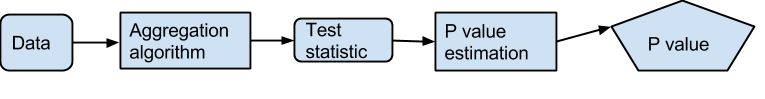
\includegraphics[width=0.8\textwidth]{statisticalTestFlow}
  \caption{Graphical representation of statistical test flow}
  \label{fig:statisticalTestFlow}
\end{figure}

Statistical tests are usually built by first gathering the necessary raw data. For example, make 80 persons run for 30 minutes and measure blood pressure before and after running. Then the data should be organized by some kind of aggregation algorithm which also might filter out samples that are not related to the hypothesis in question. For example, sorting and grouping the blood pressure results by gender and weight, in ascending order. Then filter out any group that had too few samples. A test statistic is chosen and calculated afterwards. After that a p-value can be estimated, which tells if the observable feature is interesting or not. For example, if running plays a role in raising a person`s blood pressure.

\subsubsection{Test Statistic}

The test statistic is a scalar function of all the observations, which summarizes the data by a single number. This value is used to estimate a p-value and accept or reject the hypothesis. Commonly, the test statistic is either one-sample, two-sample or paired statistic, depending on the tests.

A one-sample test investigates whether the data collectively satisfies some hypothesis, e.g. the data is generated by Gaussian distribution or has specific theoretical mean value(expected value).

A two-sample test compares two sub-populations of data, e.g. persons with high blood pressures and persons with low blood pressures.

A paired test characterizes the change of before and after measurements, e.g. does some novel medical drug treatment work. The differences between measured observable case and control experiment pairs comes from the same distribution. For instance, we might use paired statistical distance to estimate whether the differences between paired measurements are symmetrical or not. If the differences are symmetrical, then a positive difference $x$ is equally likely as a negative difference $-x$.

\subsection{Hypothesis}

\subsubsection{Null hypothesis}

In statistics, a null and alternative hypothesis are raised to find out if the test bears any interesting results. A null hypothesis in general terms means that the test results are boring or that there is no effect. It means there is no relationship between the two observed features. For example, when measuring blood pressure before and after running, the null hypothesis would state that blood pressure will not change when running.

The null hypothesis also defines the data distribution. For example, it might define that data is generated by a Gaussian distribution. Since null hypothesis is the boring result, i.e., that`s what the data set usually looks like, then generally the data will be distributed according to the null hypothesis. Since the null hypothesis defines the data distribution, it will also define the test statistic distribution. Finally, since the null hypothesis defines the data distribution and test statistic distribution, it will also play a role in estimating the p-value for the test statistic.

For example, if the observations $x_1, x_2, ..., x_n$ are generated by coin flip, then the test statistic $T=x_1 + x_2 + .. + x_n$ has a binomial distribution. With $n$ number of trials, one side of the coin always has a probability of $\frac{1}{2}$ to occur with every flip. If test statistic is defined as $T=x_1(1-x_1) + x_2(1-x_2) + ... + x_n(1-x_n)$, then it is constantly zero and thus does not hold any relevance. The exact form of the test statistic determines the properties of the test.

\subsubsection{Alternative hypothesis}
The alternative hypothesis is the opposite of to the null hypothesis. In simple terms, one could think of it as true or interesting result. It means that the two measured samples have a relationship between them, either in direct or indirect ways. A good example to explain these two is the court verdict. If null hypothesis is kept, then the suspect has not been found guilty. There was not enough evidence. On the contrary, if null hypothesis was rejected, the suspect was found guilty, because there was enough evidence to make that decision. Although the alternative hypothesis could be anything that is not a null hypothesis, some alternatives to the null hypothesis are easier to distinguish from the null hypothesis.

When the null hypothesis is true, then the test statistic has a well-defined probability distribution. This means that one can predict pretty well the possible outcome of subset of samples. For example, the alternative hypothesis can be separated from the null hypothesis if the distribution of the test statistic is vastly different from the null hypothesis. The alternative hypothesis corresponding to the null hypothesis causes the test statistic to be at the edges of a probability distributions, which makes them hard to predict.

\subsubsection{P-value}
P-value is estimated from the test statistic. It is used to find out if the test data is interesting. A certain threshold, called significance level (usually 0.05) is accepted as p-value. If the p-value is within significance level, then null hypothesis is rejected. If the p-value is below significance level, then null hypothesis is kept and the data falls into distribution as defined by null hypothesis. A variety of algorithms have been thought for p-value estimation, depending on the type of data, goals of the tests and even the amount of data. Statistics need to make the right choice between the algorithms by taking all these assumptions into an account.

The p-value can be either one-sided or two-sided. Given a test statistic $T_0$ which we computed from observed data. A one-sided p-value shows the probability that we can get a value $T$ that is larger or equal than the $T_0$ in the distribution defined by $H_0$. This can be seen visually in Figure ~\ref{fig:p_value_one_sided}.

\begin{figure}[H]
  \centering
  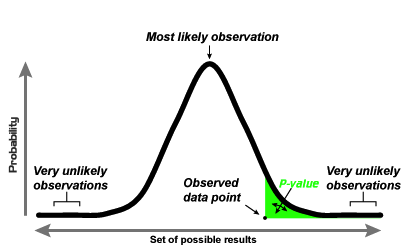
\includegraphics[width=0.4\textwidth]{p_value_one_sided}
  \caption{One sided p-value representation. A p-value(shaded green area) is the probability of an observed (or more extreme) result arising by chance. ~\cite{p_value_pic_cite}}
  \label{fig:p_value_one_sided}
\end{figure}

A two-sided p-value shows the probability that we can get a value $T$ that is larger or smaller than the $T_0$ in the distribution defined by $H_0$. This can be seen visually in the Figure ~\ref{fig:p_value_two_sided}.

\begin{figure}[H]
  \centering
  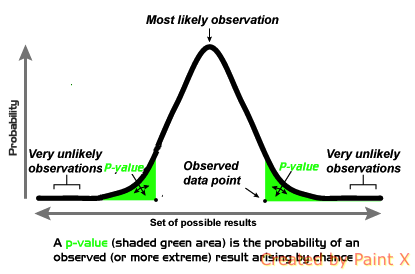
\includegraphics[width=0.4\textwidth]{p_value_two_sided}
  \caption{Two sided p-value representation. A p-value(shaded green area) is the probability of an observed (or more extreme) result arising by chance. ~\cite{p_value_pic_cite}}
  \label{fig:p_value_two_sided}
\end{figure}

\subsection{Wilcoxon test}

The Wilcoxon signed-rank test is a statistical hypothesis test that is used when comparing two related samples, matched samples, or repeated measurements on a single sample. This means that with Wilcoxon test you can look at some measurable feature, e.g. blood pressure. If two or more experiments in different conditions have been made on it,e.g. gene experiments and their confirmation results, Wilcoxon test can be used to see if the changes of the measurement levels are relevant. The null hypothesis $H_0$ means that the difference between pairs is zero. The alternative $H_1$ means that it is different from zero.

It was popularized by Sidney Siegel in his book ``Nonparametric statistics - for the behavioral sciences". Sidney used the symbol $T$, to denote test statistic. Because of this, the test is sometimes referred to as the Wilcoxon $T$ test. However, in this paper the more common $W$ is used to represent the Wilcoxon test statistic value.

\subsection{Wilcoxon test assumptions}

\begin{enumerate}
  \item Two measurements can always be compared and thus ordered. For example, measurements are real values or ordered categorical values
  \item Measurements can be naturally paired into case-control or before-after experiments. For example, measurements of patient`s white blood cell levels before and after treatment.
  \item All measurement pairs are independent from other pairs. For example, measurement of one individual does not influence the other. In medicine studies, the patients are sampled randomly. There is no evident procedure in selecting patients or no planned action to organize a study so one could get the ``desired'' result.
\end{enumerate}

\subsection{How to compute}
Let $N$ be the sample size, the number of pairs. Then we can use the following variable to compute the $W$ test. \\For $i=1,...,N$, let $x_{1, i}$ and $x_{2, i}$ of the same quantity in case and control group denote the measurements. \\
Let $W$ be the Wilcoxon test statistic. \\
Let $z$-score be the Wilcoxon test standard score. \\
Let $N_0$ be the number of pairs from which onward we can approximate the p-value. This value is currently undefined and is the focus of this paper. It will be discussed in the future chapters.

The computation of the statistic W is organized into five steps. The last step diverges into two possible paths and the choice of the path that is chosen depends whether $N  >= N_0$.

\begin{enumerate}
\item
For $i=1, .., N$, calculate $|x_{2,i} - x_{1,i}|$ and $\sign(x_{2,1} - x_{1,i})$, where $\sign(x)$ is the sign function.
\item
Order the $N$ pairs from smallest absolute difference to largest absolute difference, $|x_{2,i} - x_{1,i}|$.
\item
Rank the pairs, starting with the smallest as $1$. Ties receive the rank equal to the average of the ranks they span. Let $R_i$ denote the rank.
\item
Calculate the test statistic $W$, the absolute value of the sum of the signed ranks.
\begin{equation}
  W= \left|  \sum\limits_{i=1}^{N} \left[ \sign(x_{2,i} - x_{1,i})R_i \right] \right|
\end{equation}

\item
As $N$ increases, the sampling distribution of $W$ converges to a Gaussian distribution. Where $N_0$ depends on how accurate you want your results to be.
\begin{enumerate}
\item
For $N \geq N_0$, a $z$-score can be calculated as
\begin{equation}
  z=\frac{W-0.5}{\sigma_w}
\end{equation}
\begin{equation}
  \sigma_w = \sqrt{\frac{N(N + 1)(2N + 1)}{6}}
\end{equation}

If $Z > Zcritical$ then reject $H_0$, where $Z_{critical}$ is calculated with Gaussian distribution.

\item
For $N < N_0$, $W$ and $N$ is used to calculate accurate $P$ value as described in Section ~\ref{sec:v_p_table_formulas}.

If $ P \geq P_{critical}$, $N$ then reject $H_0$
\end{enumerate}
\end{enumerate}

\subsection{Example}
Given pairs of measurements $(6, 8), (2, -3), (-3, 3), (1, 3)$.

\begin{enumerate}
\item Calculate absolute values and signs of the pairs. For example, $(6, 8)$ value becomes $2$ and sign $-1$.
\item Order the pairs. Ties receive the rank equal to average of the ranks they span. Let $R_i$ be the rank value.
\item Calculate the test statistic W.
\item Since $N_r$ is very small, use a table to look up the $p$ value. The calculation of $p$ table is shown in Section ~\ref{sec:v_p_table_formulas}. \\
$P(5, 4) = 0.3125$ \\
Since $0.3125 > 0.05$, reject $H_1$
\end{enumerate}

The calculations can also be seen on Table ~\ref{table:wilx_example}.

\begin{table}[h!]
  \begin{center}
    \begin{tabular}{ccccccc}
      \hline
      i & $x_{2, 1}$ & $x_{1, i}$ & $\sign$ & abs & $R_i$ & $\sign * R_i$\\
      \hline
      1 & 6 & 8 & 1 & 2 & 1.5 & 1.5 \\
      \hline
      2 & 2 & -3 & -1 & 5 & 3 & -3 \\
      \hline
      3 & -3 & 3 & 1 & 6 & 4 & 4 \\
      \hline
      4 & 1 & 3 & 11 & 2 & 1.5 & 1.5 \\
      \hline
    \end{tabular}
    \caption{Initial data}
    \label{table:wilx_example}
  \end{center}
\end{table}


\subsection{P-value assignment}
Let us consider Wilcoxon test if we have 6 measurements. Then there are three differences as shown in in Figure ~\ref{fig:patientExample}. As the test considers only the sign and order of the measurements, then only 8 configurations are possible as shown in Table ~\ref{table:adding_w_results}. Due to the symmetry of the possible configurations under the distribution of the null hypothesis, all 8 configurations can be proven equally probable.
\begin{figure}[h!]
  \centering
  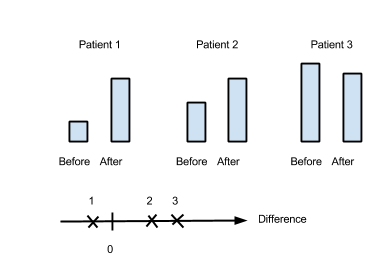
\includegraphics[width=0.8\textwidth]{patientExample}
  \caption{Patient example}
  \label{fig:patientExample}
\end{figure}

Now if the W value in our data is $+2$, then there are 3 configurations that have larger or equal W value. This can be seen from the Table ~\ref{table:adding_w_results}. Then the one-sided p-value is $\frac{3}{8}$. The two-sided p-value is $\frac{3}{4}$. The same procedure is needed to assign p-value.

\begin{table}
  \begin{center}
    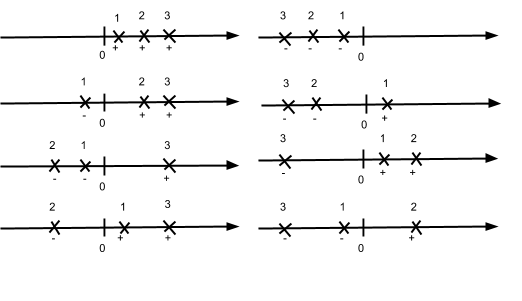
\includegraphics[width=0.8\textwidth]{rankSignsExample}\\
    \begin{align*}
        W&= 1 + 2 + 3 = 6 & W&=-1 - 2 - 3 = -6\\
        W&= -1 + 2 + 3 = 4 & W&= 1 - 2 - 3 = -4\\
        W&= -1 - 2 + 3 = 0 & W&= 1 + 2 - 3 = 0\\
        W&= 1 - 2 + 3 = 2 & W&= -1 + 2 - 3 = -2\\
    \end{align*}
    \caption{The figure shows all possible configurations of differences. The equations show values of the test statistic corresponding to the configurations.}
    \label{table:adding_w_results}
  \end{center}
\end{table}

Wilcoxon test neglects the actual value of the tests. To estimate the p-value, we only need to know the $W$ value and number of tests $N$. $W$ statistic will always create the same configuration for each possible $N$.

\subsubsection{Exact computation of P-value}
\label{sec:exact_computation_of_p-value}
In general, we get $2^n$ equally probable configurations of differences and assigning a $p$-value can be reduced to the following problem. Given a $N$ ranks, we assign + or - sign to each rank randomly and each sign has equal probability to be assigned. We can consider all $2^n$ possible sign assignments and find out in how many ways we can assign the ranks to get a certain sum $k$. If we do this for every possible $k$, then a $V$-array is formed. It signifies all the possible random signed rank combination sums in an $N$ sized ranked array, where $k$ shows how many times a certain sum was achieved. If we calculate $V$-array for every possible number of ranks up to the fixed $N$, then a $V$-table is formed which we can use through $V_{N, k}$ to find out how many times a certain sum $k$ was achieved.

From this table, the probability that $W\geq k$ can be calculated. This value will show that given $N$ ranks with random signs, how probable it is that a sum $k$ is the result. If this process of calculating values is done repeatedly for every possible $N$ and $k$, then a $P$-table forms. The $P$-table shows the probability of every possible sum $k$ appearing given $N$ ranks with random signs. Let $P_{N, k}$ be the function to get the desired $P$ value from that table.

If the $P$-table gets large enough, it will start taking the shape of Guassian distribution. Because of that, given enough ranks, a Gaussian distribution can be used to approximate the $P$-table.

\subsubsection{The V and P table formulas}
\label{sec:v_p_table_formulas}

Given $N$ which shows us the number of ranks starting from $0$ and $k$ which shows us the sum that we are interested in. Recursively apply this algorithm until you reach to the $N = 1$.

\begin{equation}
  V_{N+1, k} = V_{N, k-1} + V_{N, k+N+1}
\end{equation}

There are some additional conditions to the formula:

\begin{equation}
V_{N, k} = 0  \quad\text{if}\quad k <  \frac{-N(N+1)}{2} \quad\text{or}\quad k >  \frac{N(N+1)}{2}
\end{equation}

\begin{equation}
V_{N, k} = 1 \quad\text{if}\quad k =  \frac{ -N(N+1)}{2} \quad\text{or}\quad k =  \frac{N(N+1)}{2}
\end{equation}

With these formulas, the probability that $W$ is a certain value can be calculated.

Given $V$ table, $N$ and $k$, we can calculate the $P$ as follows.

\begin{equation}
P(T) = \frac{1}{2^n} \cdot \abs{\sum\limits_{K=T}^{\infty}{W_{N,K}}}
\end{equation}

To get the P table, we go through all $N$ and $K$ values that we are interested in.

As a concrete example, consider the case where $N=2$, then ranks are ${0, 1, 2}$, one can combine them as follows.
\begin{align*}
0 + 1 + 2 \\
0 + 1 - 2\\
0 - 1 + 2\\
0 - 1 - 2
\end{align*}
This gives us one way to get $3$, one way to get $1$, one way to get $-1$ and one way to get $-3$. It can now be calculated that there is $0.25\%$ probability that our value is $3$ or lower and $0.5\%$ probability that our value is $1$ or lower.

\subsubsection{The Gaussian approximation of P table}
As mentioned above, if the number of ranks $N$ gets large enough, then Gaussian distribution can be used. To use that, the cumulative density function $F(x)$ is usually used. A simple Gaussian function $F(x, 1)$, where $x$ is the statistic $z$-value, e.g. standard score and $1$ is the sigma, will give approximately the same results as the accurate $P$ table.

\subsubsection{Code sample}
A python code to calculate the V table is as follows.
\begin{verbatim}
def V(n, k, vTable):
    if((n == 1 and (k == 1 or k == -1)) or (n == 0 and k == 0)):
        return 1
    if((k < -(n * (n + 1) / 2)) or (k > (n * (n + 1) / 2))):
        return 0
    n = n - 1

    kIndex =  k + kSize

    leftValue = 0 if kIndex - n - 1 < 0 or \
      kIndex - n - 1 >= len(vTable[n]) else vTable[n][kIndex - n - 1]
    rightValue = 0 if kIndex + n + 1 < 0 or \
      kIndex + n + 1 >= len(vTable[n]) else vTable[n][kIndex + n + 1]

    return leftValue + rightValue

def calculateVValues():
    vTable = []
    for n in range (nSize):
        tableRow = []
        for T0 in range (kSize * 2 + 1):
            tableRow.append(V(n, T0 - kSize, vTable))
        vTable.append(tableRow)
    return vTable

\end{verbatim}

The python code to calculate the P table is as follows:

\begin{verbatim}
def calculatePValues(vTable):
    pTable = []
    for n in range(nSize):
        tableRow = []
        sumValue = 0
        powerValue = 2**n
        for T0 in range (kSize * 2, kSize-1, -1):
            sumValue += vTable[n][T0]
            p = sumValue / powerValue
            tableRow.insert(0, p)
        pTable.append(tableRow)
    return pTable

\end{verbatim}

You can find a python implementation of a code sample in repository ~\cite{stenver_repo_p_accurate_table_py}

\subsubsection{Bonferroni correction}

If you make multiple hypothesis on a test, then you increase the risk in which you reject null hypotheses when its actually true. The Bonferroni test helps to counteract this in a simple and naive way. For each hypothesis you make on a test, you should use a significance level $M$ times lower than before. This ensures that the increased risk in which we can reject null hypothesis will not raise, no matter the number of hypothesis on a test. So for example, if you make $M$ hypothesis and want a significance level $\alpha$,  then you should run each test at a significance level of $\frac{\alpha}{M}$.

If you want to use Bonferroni correction with Wilcoxon signed-rank test, then you need to keep in mind that the approximated $P$ value significance level needs to be much more accurate, since the Bonferroni test divides it by the amount of features tested. This means higher the $N_0$ value, the more features you add in the test.

\newpage

\section{Approximating the p-value}
\label{sec:approximating_p_value}

\subsection{Motivation}

The current implementations of Wilcoxon signed-rank test usually assume that $p$-value distribution is sufficiently close to Gaussian distribution, so that we can use $Z$ to calculate the $P$ value. They draw this conclusion from the assumption that the number of samples $N$ is sufficiently large to use $Z$. When $N = 1$, then approximation is quite inaccurate. As number of samples increases, then the approximation becomes more and more accurate on absolute scale. When the $N->\infty$, then the $P_{approx}$ approximate region will almost equal the $P$ accurate region, which also means that the region will be almost perfect Gaussian Distribution. This means that when $N->\infty$, then there is no reason not to use Gaussian Distribution, as it will be almost completely accurate, except at the very edges. This allows them to use Gaussian Distributions to approximate the p-value and the accurate $P$ table calculation is often left unoptimized.

In the BIIT research group, and many others, the $N$ is usually not sufficiently large. This means that Gaussian distribution cannot be used. Also, since BIIT uses multiple hypothesis testing, the approximation must be good even at the very edges of distribution. As mentioned above, the Bonferroni correction will lower the significance level significantly as $N$ rises. Furthermore, it is not known where exactly the $N$ limit is, so an arbitrary number is used for that purpose. The textbooks~\cite{lowry_concepts} currently suggest a sufficient $N$ is 10. In this work we studied the question whether this assumption is justified in detail.

The approximation is computationally cheap and the preferred method to be used over accurate $P$ table, which is computationally expensive. Because of this, one focus of the paper is finding out how good the approximation of Gaussian Distribution is and finding out the exact $N$ where we can use approximation instead on accurate $P$ table while maintaining a high enough accuracy. Let $N_0$ be high enough $N$, which allows us to use approximation accurately.

The bottlenecks of the other implementations of the Wilcoxon test is, when $N$ is low, but the number of tests is high. In this case they calculate the $P$ and $V$ tables every time the test is run, thus if you run thousands of tests in a row, a lot of complex recomputation is done. This eventually becomes a performance issue. To speed this up - this project will calculate the entire $P_{N, k}$ for every value that is possible where $N < N_0$. Then the $P_{N, k}$ will be hardcoded inside the program for quick lookup of the value.


\subsection{When can we approximate}
The relative and absolute error behave very differently. The absolute error is calculated as follows.
\begin{equation}
  \Delta = P_{k, N} - P_{approx, k, N}
\end{equation}
The relative error is calculated as follows.
\begin{equation}\label{eq:relative_error}
  \epsilon = \frac{\Delta}{P_{approx, k, N}} \cdot 100\%
\end{equation}
Note that the errors are signed, because this lets us know if the p-value estimation is over- or underestimated.
The absolute error between accurate table values $P$ and approximate table $P_{approx}$ values first falls and then rises until at the center of the distribution, but gets stable and almost constant from the middle to the edge of the distribution. It can be seen on the Figure ~\ref{fig:absolute_difference}. Note that the error fluctuates. This is artifact of the V-table quickly fluctuating values that the smooth approximation cannot follow. The Relative error gets smaller, the higher the number of samples $N$ is. However, the relative error looks like a slide. It is stable at the center of the distribution, but starts rising sharply at the middle. At the edge of the distribution, the relative error is nearly 100\%. It can be seen at the Figure ~\ref{fig:epsilon_difference}.

\begin{figure}[H]
  \centering
  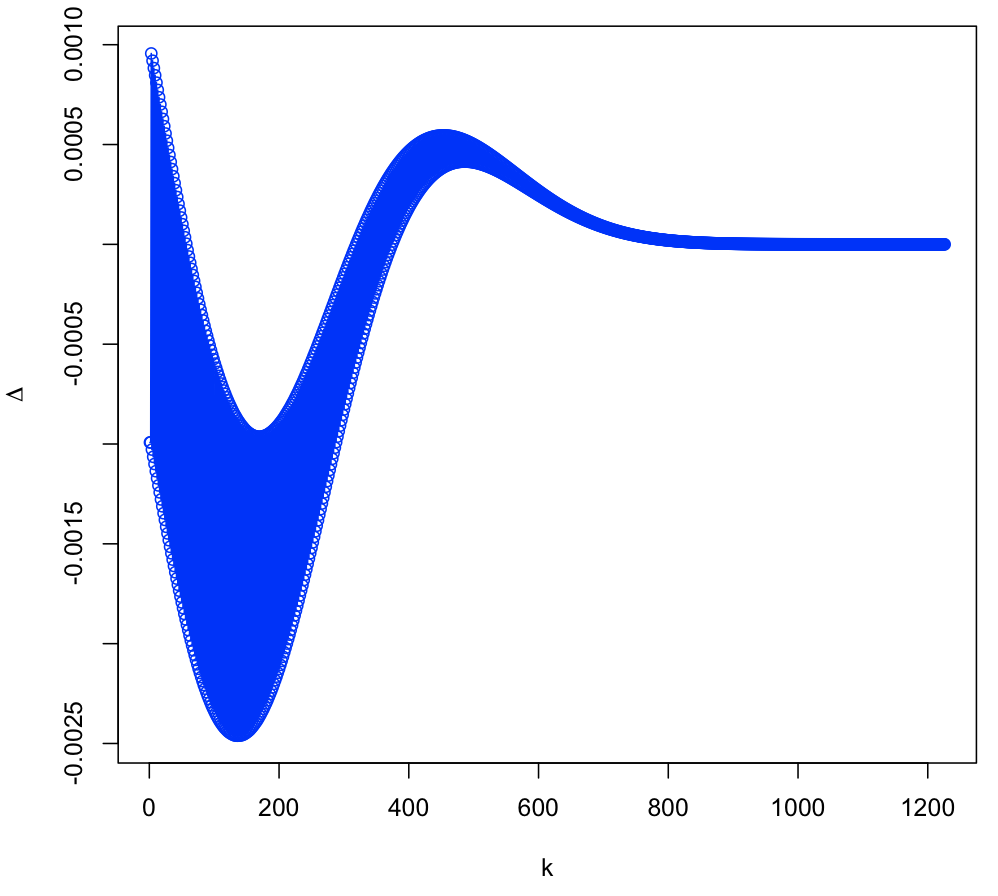
\includegraphics[width=0.8\textwidth]{approximate_accurate_difference}
  \caption{Absolute error between accurate $P$ and approximate $P_{approx}$ values for sample size $N=50$.}
  \label{fig:absolute_difference}
\end{figure}

\begin{figure}[H]
  \centering
  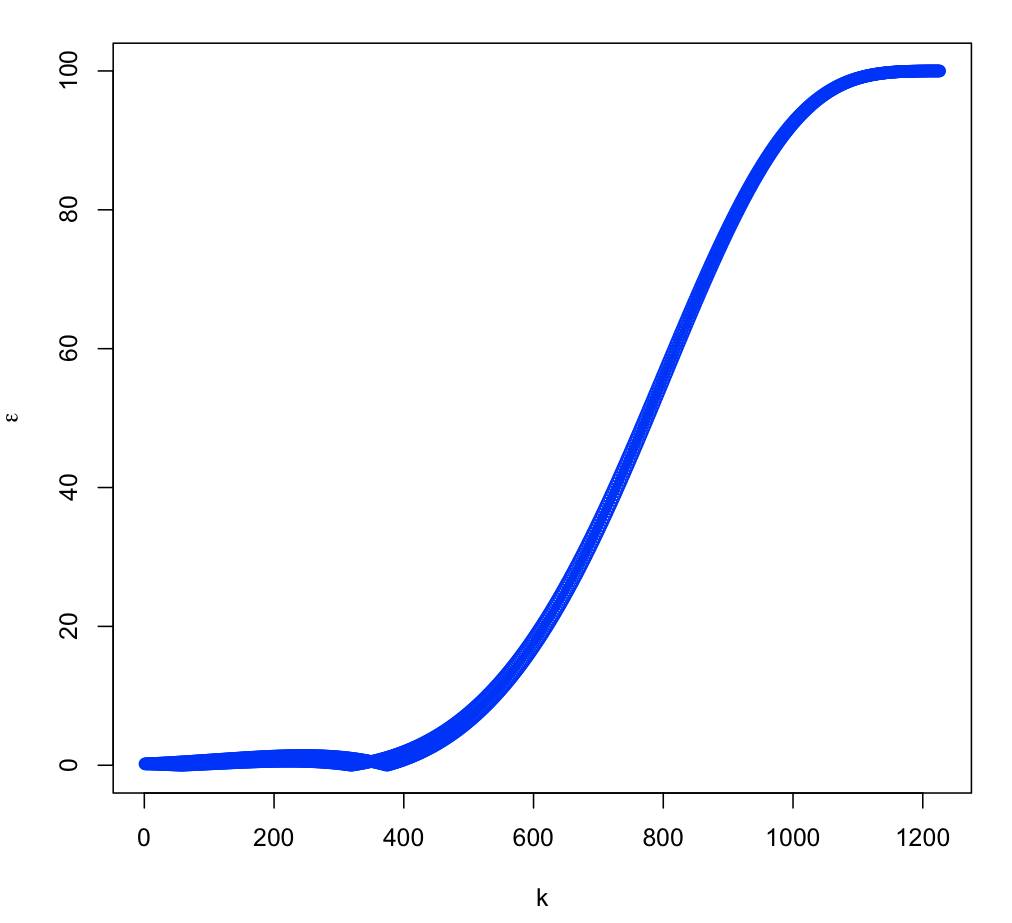
\includegraphics[width=0.8\textwidth]{approximate_accurate_epsilon}
  \caption{Relative error between accurate $P$ and approximate $P_{approx}$ values for sample size $N=50$.}
  \label{fig:epsilon_difference}
\end{figure}

It is important to have low relative error on the region, i.e., good region, because this ensures that the test results stay accurate. If the relative error is high, then this will also increase the possibility of a false positive, that is, rejecting $H_0$ when we actually should not.

First we wanted to confirm that as the number of samples grows, accurate table values $P$ and approximate table values $P_{approx}$ will get become more similar. To do this, we used the following equation for each $N$.

\begin{equation}
  k_0 = \max_k \{ k: P_{N, k} > 0 \}
\end{equation}

And compared them to the results as shown in the equation below, where $\epsilon_k$ is the relative error with the corresponding $k$ value as shown in the equation ~\eqref{eq:relative_error}.
\begin{equation}
  k_1 = \max_k \{ k: \epsilon_k \leq 5\% \}
\end{equation}

The results of the table can be seen on Figure ~\ref{fig:T0vsN}.

\begin{figure}[H]
	\centering
  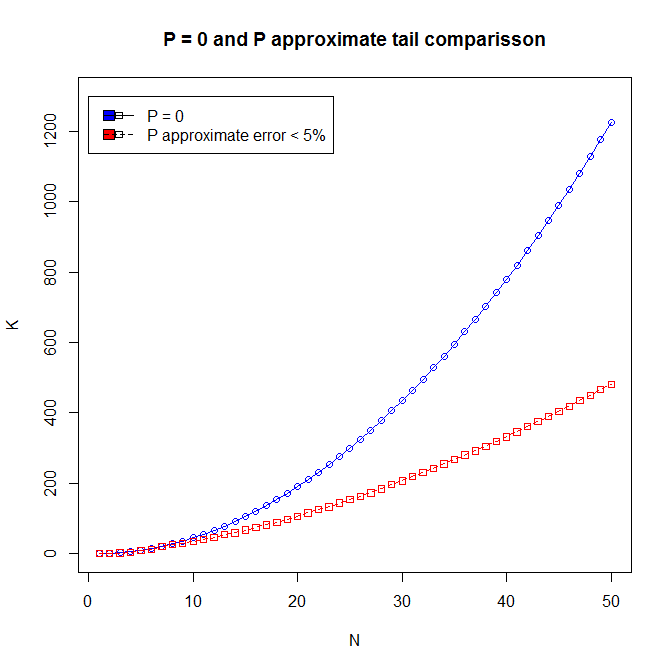
\includegraphics[width=0.8\textwidth]{T0vsN}
	\caption{Region between low relative error and actual distribution edge increasing as sample size increases.}
	\label{fig:T0vsN}
\end{figure}

Much to our surprise, as $N$ grew, the gap between approximate and accurate values grew bigger. This meant that as $N$ grows, the relative approximate error of Gaussian distribution will get more inaccurate toward the tails of the distribution. Previously we thought that with the growth of $N$, Gaussian would surely get more and more accurate.
From Figure ~\ref{fig:PandPapproxAsKincreases} we cant really make a difference between accurate $P$ and approximate $P_{approx}$ values, but if we put the values to logarithmic scale, the difference is easier to spot. From Figure ~\ref{fig:logPlogPapproxAsKincreases} we can see that approximated $P_{approx}$ values are a little bit bigger toward the edge of distribution - as can be seen when $K$ grows.

\begin{figure}[H]
  \centering
  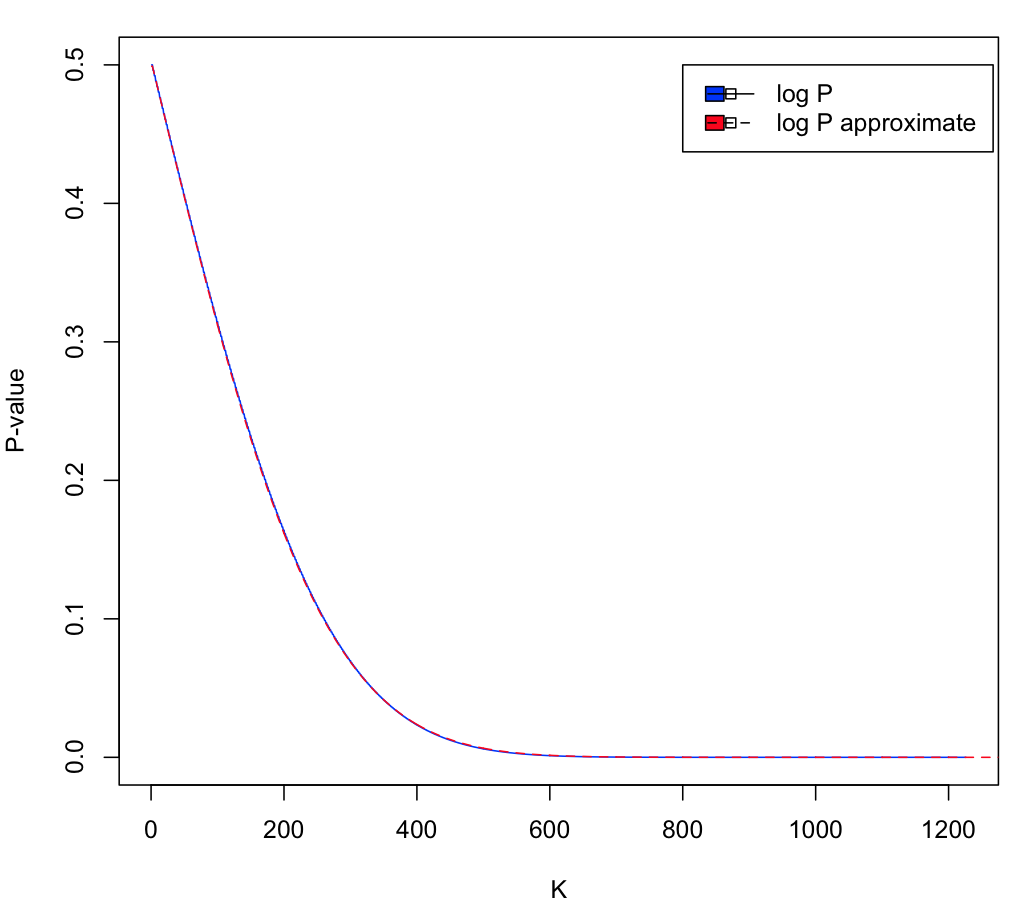
\includegraphics[width=0.6\textwidth]{PandPapproxAsKincreases}
  \caption{Accurate $P$ and approximate $P_{approx}$ values as $k$ increases when sample size $N=40$.}
  \label{fig:PandPapproxAsKincreases}
\end{figure}

\begin{figure}[H]
  \centering
  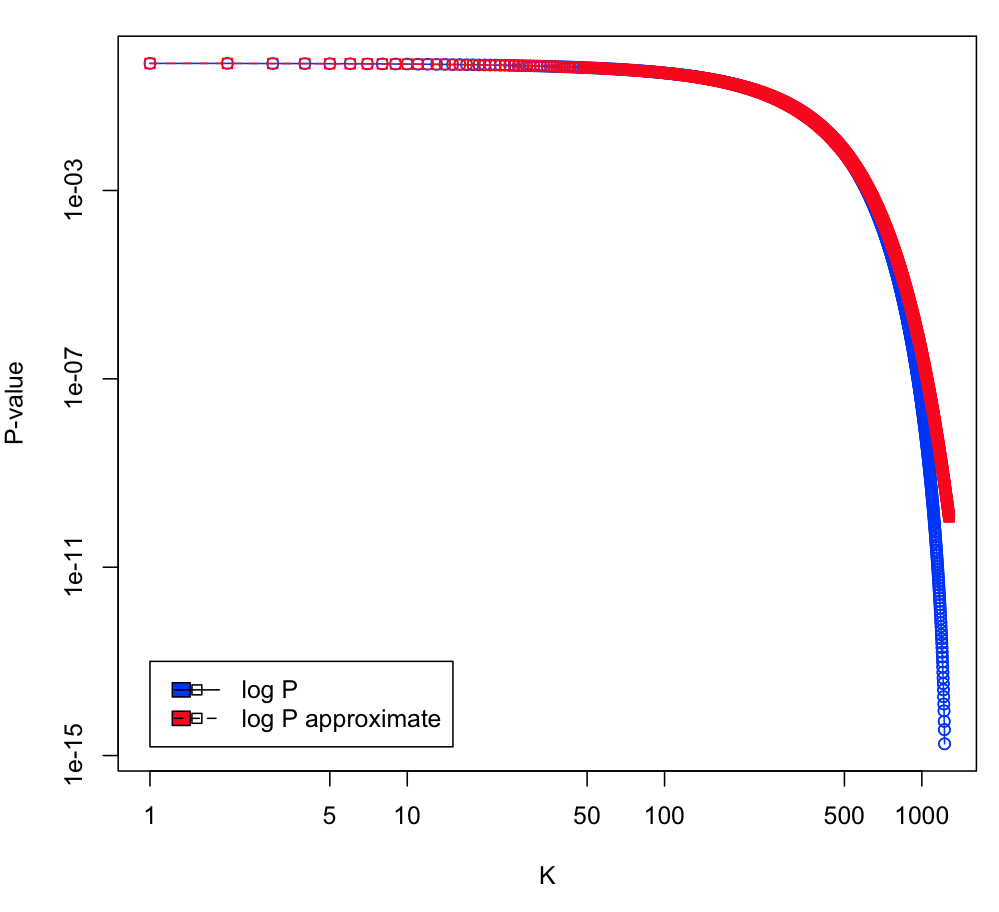
\includegraphics[width=0.6\textwidth]{logPlogPapproxAsKincreases}
  \caption{Logarithmic accurate $P$ and approximate $P_{approx}$ values as logarithmic $K$ increases when sample size $N=40$.}
  \label{fig:logPlogPapproxAsKincreases}
\end{figure}

To further investigate this finding, we decided to find out the minimum approximate $P$ value that we can get for each $N$ while maintaining a certain relative error $\epsilon$ threshold. For that we first find the set.
\begin{equation}
K={k: \epsilon_k < \textit{threshold}}
\end{equation}
Then we choose the minimal approximate $P$ value.
\begin{equation}
p = min{P_{approx, k}: k \in K}
\end{equation}

The thresholds chosen were $\epsilon=5\%, \epsilon=10\%, \epsilon=20\%, \epsilon=50\%$. From Figure ~\ref{fig:PvsN} we can see that as the $N$ grows, the graph becomes stable, meaning that the distribution becomes a Gaussian distribution at around $N > 10$ and $N < 25$.  When $N < 10$, then the approximation is so random that it cannot be used reliably. For example, if $N=30$, we can read form this graph that relative error $\epsilon<5\%$ is attainable only for p-values that are larger than $0.012$. We can also see from the figure that relative error $\epsilon$ does not increase monotonically when $k$ grows, thats why there are fluctuations on the graph.We can see that the minimum $P$ value under error threshold does get smaller, as $N$ increases, so this further proves that Gaussian distribution does get more accurate as $N$ grows. This is because as $N$ increases, we can take a $P$ value closer to the tail of the distribution and still get an accurate value.

\begin{figure}[H]
  \centering
  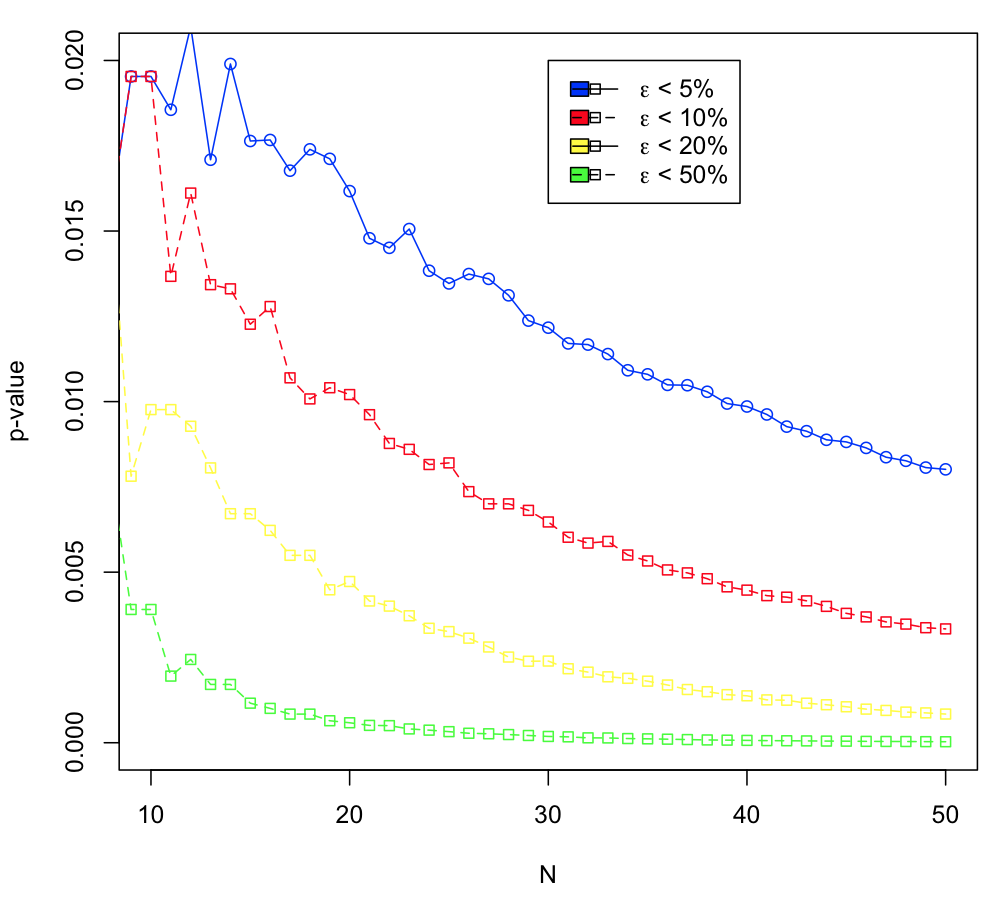
\includegraphics[width=0.8\textwidth]{PvsN}
  \caption{Relative error $\epsilon$ as sample size $N$ increases}
  \label{fig:PvsN}
\end{figure}

The Figure ~\ref{fig:RelativeErrorDecresingPgrows} shows us the relative error as $P$ grows when $N = 20$. The $P$ values are logged on this graph. There are two noteworthy things here, however. First, around $P = 0.05$, the relative error actually gets a little small tip toward accuracy. Second, it can be seen that there are two accuracy paths that the error takes, depending on weather in $P_{approx N, K}$  the $K$ is even or odd number. This is a computational artifact caused by the recurrence of the $V_{N, K}$ values and we will not make any conclusions of that. To understand this better, once must familiarize himself with the algorithm defined in the Chapter ~\ref{sec:v_p_table_formulas}.


\begin{figure}[H]
	\centering
  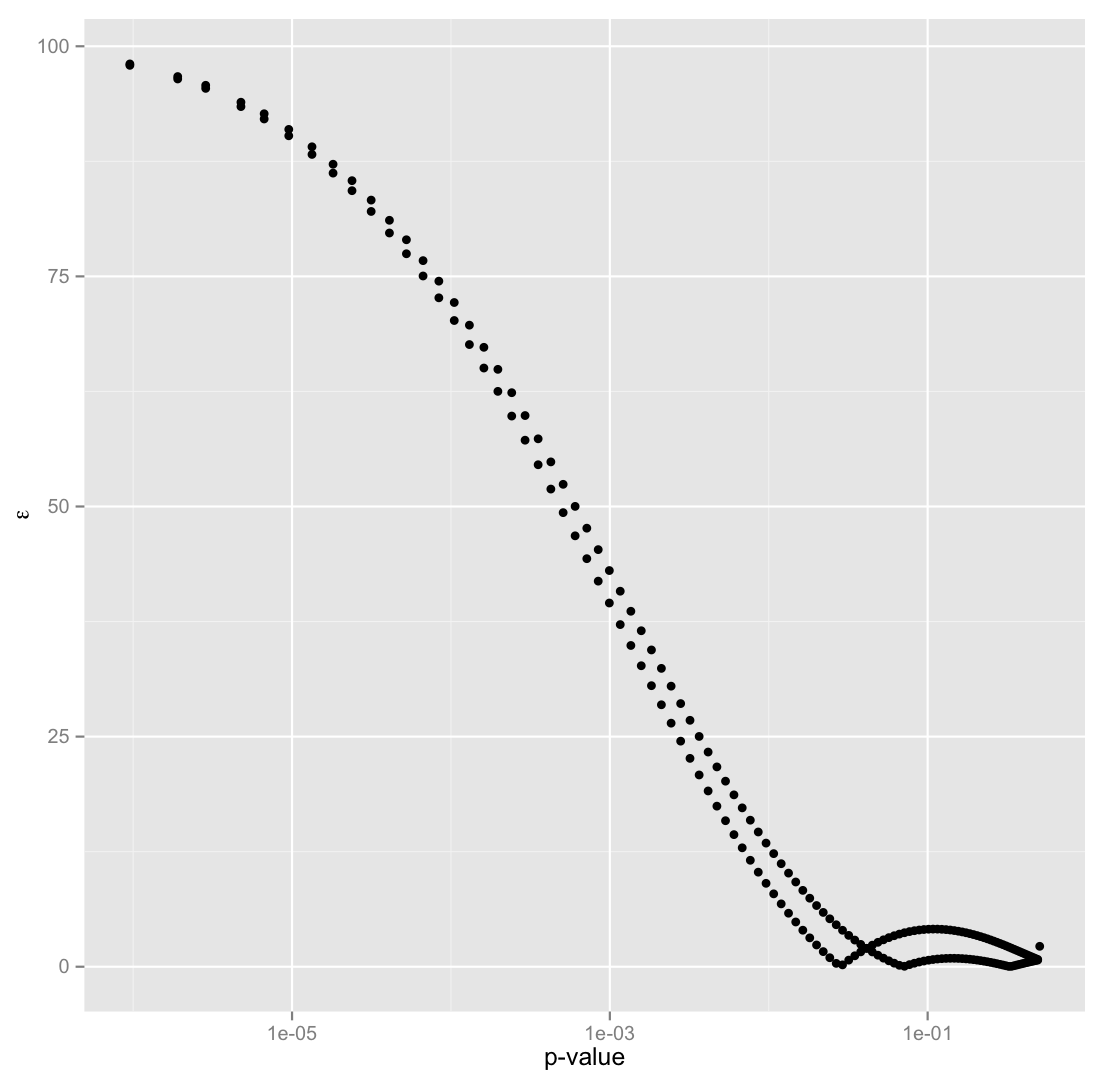
\includegraphics[width=0.8\textwidth]{RelativeErrorDecreasingPgrowsN20}
	\caption{Relative error $\epsilon$ decreasing as p-value grows, when $N=20$}
	\label{fig:RelativeErrorDecresingPgrows}
\end{figure}

\subsection{The behaviour of relative error}
To further prove that we can start using Gaussian Distribution at a certain $N$, we needed to prove that $P_{approx}$ will get more accurate as the $N$ increases toward the tail of the distribution as-well. To achieve this, we found out the largest relative error $\epsilon$ between $P$ and $P_{approx}$ for each $N$ and for each p-value in the regions $[1, 0.1], [0.1, 0.01], ... , [\frac{1}{10^{6}};\frac{1}{10^{7}}]$. As can be seen from Figure ~\ref{fig:LargestApproxPRelativeError0_100} and Figure ~\ref{fig:LargestApproxPRelativeError100_500}, the relative error increases fast. When p-value is between $10^{-5}$ and $10^{-6}$ the relative error is massive. When $N=200$, then the error is still around $40\%$. The bigger the $N$ gets, the bigger the error at the tail. However, it can also be seen that the relative error decreases steadily as $N$ grows for each of the p-value ranges chosen. This means that even though the error of the distribution tail edge does increase as $N$ grows, the approximate $P_{approx}$ and accurate $P$ values do get more similar as the $N$ grows.

\begin{figure}[H]
  \centering
  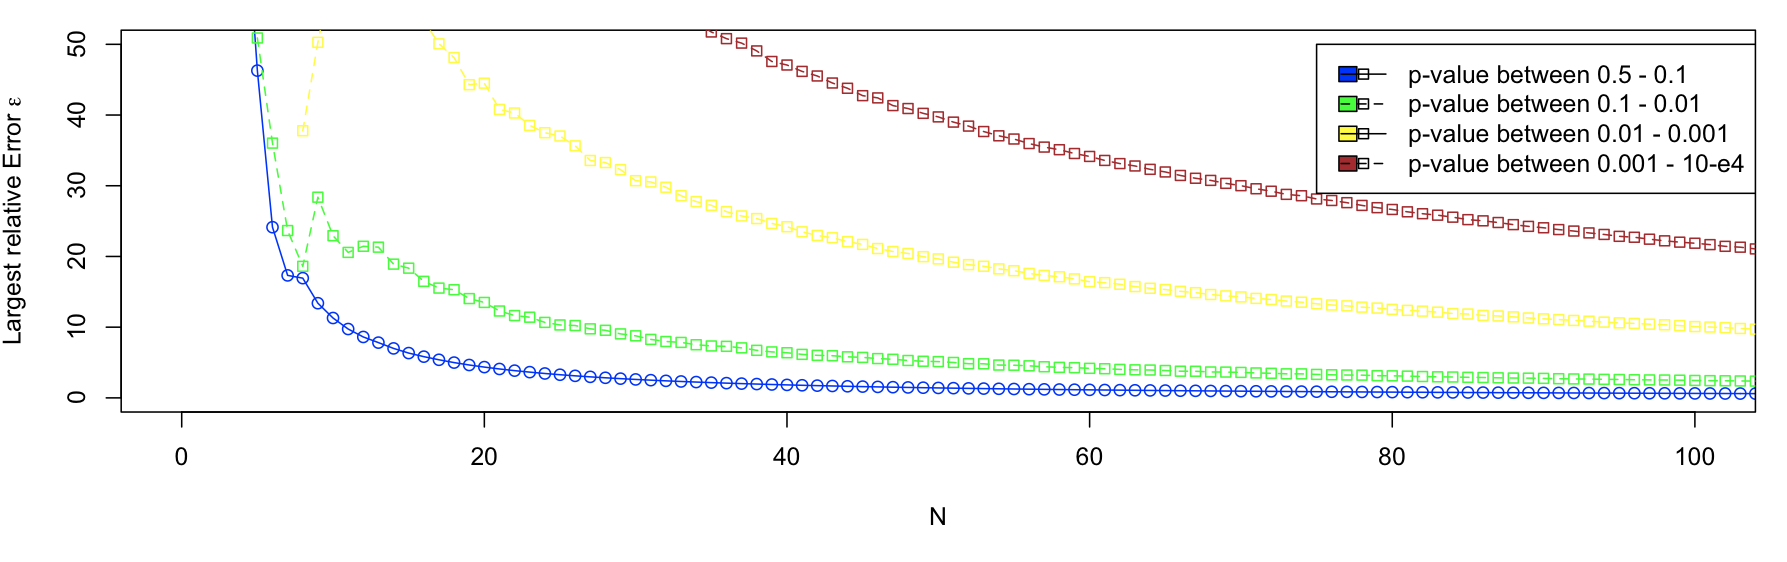
\includegraphics[width=1\textwidth]{LargestApproxPRelativeError0_100}
  \caption{Showing the maximum relative error $\epsilon$ decreasing in probability ranges, as sample size $N$ increases}
  \label{fig:LargestApproxPRelativeError0_100}
\end{figure}

\begin{figure}[H]
  \centering
  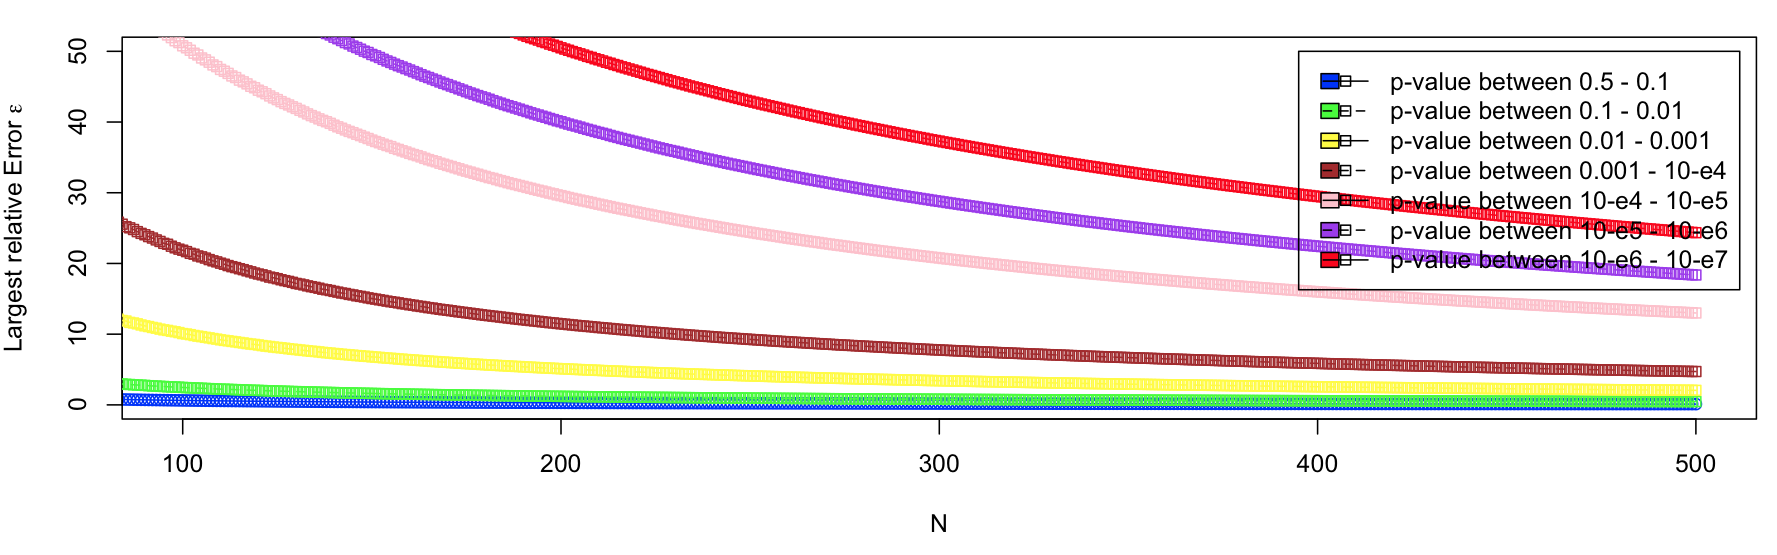
\includegraphics[width=1\textwidth]{LargestApproxPRelativeError100_500}
  \caption{Showing the maximum relative error $\epsilon$ decreasing in probability ranges, as sample size $N$ increases, when axises are log scaled}
  \label{fig:LargestApproxPRelativeError100_500}
\end{figure}

\newpage

To investigate the relation between accurate $P$ and approximate $P_{approx}$ values, we wanted to see the difference between all p-values values when $N = 50$ and when $N = 25$. As can be seen from Figure ~\ref{fig:PvsP50} or Figure ~\ref{fig:PvsP25}, the $P_{approx}$
is constantly a little bit larger. When $N = 25$, the graph is a little less smooth than when $N=50$. This follows the same story as before - the bigger the $N$, the more similar the p-values.

\begin{figure}[H]
  \centering
  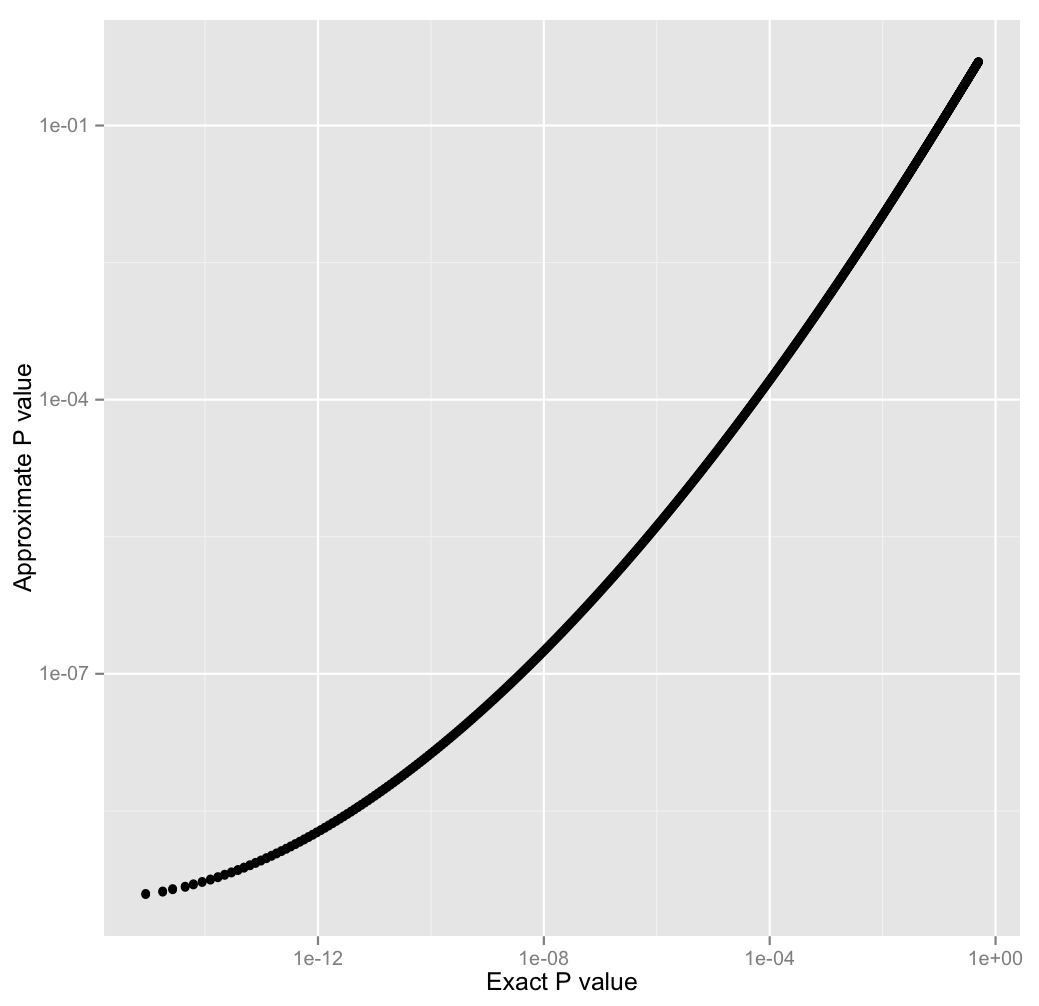
\includegraphics[width=0.8\textwidth]{PvsP50}
  \caption{Relative value of all accurate $P$ and approximated $P_{approx}$ values when sample size $N$ is 50}
  \label{fig:PvsP50}
\end{figure}

\begin{figure}[H]
  \centering
  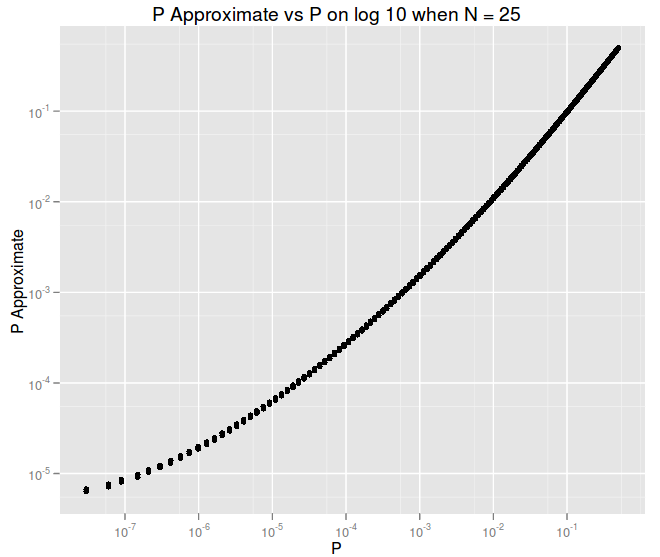
\includegraphics[width=0.8\textwidth]{PvsP25}
  \caption{Relative value of all accurate $P$ and approximated $P_{approx}$ values when sample size $N$ is 25}
  \label{fig:PvsP25}
\end{figure}

\subsection{Finding out when can we approximate p-value}
Judging by all the data that has been gathered, it be can clearly see that as $N$ grows, accurate $P$ and approximate $P_{approx}$ values grow apart at the edges of distribution. Nevertheless, overall the distribution gets more and more similar. The most helpful graphs to help us determine the necessary number of samples $N_0$ we need to approximate p-value is Figure ~\ref{fig:LargestApproxPRelativeError100_500}. Table ~\ref{table:requiredN} illustrates the number of samples $N$ needed for a certain relative accuracy. So the number of samples $N_0$ we need to approximate depends on the number of measurements and the required accuracy.

\begin{table}[H]
	\begin{center}
		\caption{Showing the minimal required sample size for a certain relative error and number of measurements}
	    \begin{tabular}{| l | l | l |}
	    \hline
		Measurements & Error & Required N \\
		\hline
		10 & 5\% & 25 \\
    \hline
		100 & 5\% & 250 \\
    \hline
		1000 & 5\% & 500 \\
    \hline
		10000 & 5\% & $>500$ \\
    \hline
		100000 & 5\% & $> 500$ \\
    \hline
		\hline
		10  & 10\% & 80 \\
    \hline
		100 & 10\% & 200 \\
    \hline
		1000 & 10\% & $>500$ \\
    \hline
		10000 & 10\% & $>500$ \\
    \hline
		100000  & 10\% & $>500$ \\
		\hline
    \hline
		10  & 20\% & 50 \\
    \hline
		100 & 20\% & 100 \\
    \hline
		1000  & 20\% & 280 \\
    \hline
		10000  & 20\% & 500 \\
    \hline
		100000  & 20\% & $>500$ \\
    \hline
    \hline
		10  & 50\% &  25 \\
    \hline
		100 & 50\% & 50 \\
    \hline
		1000 & 50\% & 100 \\
    \hline
		10000 & 50\% & 150 \\
    \hline
		100000 & 50\% & 200 \\
		\hline
		\end{tabular}
		\label{table:requiredN}
	\end{center}
\end{table}

\section{Further optimizations}
At the beginning of this chapter, we raised the goal of optimizing our implementation on Wilcoxon test by hardcoding the accurate $P$ value table $P_{N, K}$, so the program would not need to recompute it all the time. When given $N = 80$, then the table $P_{N, K}$ size was 2.5 MB. As pointed out in the beginning, when the $N$ grows, the table $P_{N, k}$ size grows with it with the speed $O(n^2)$. At $N = 500$, the file size was over 10 GB. This raised the need to optimize the table $P_{N, k}$ further.

As the research found out, the required sample size $N_0$ to approximate p-value was very large and thus the corresponding p-value table is really large. To make it more practical, we need a way to pack the p-value table further. For that we used several methods. We noticed that the equation ~\eqref{eq:p_div_p_approx} is 1 until around the middle-range of the $P$ value table.
\begin{equation}\label{eq:p_div_p_approx}
  \frac{P_{k, N}}{P_{approx, k, N}}
\end{equation}
Hence it makes sense to approximate equation ~\eqref{eq:p_div_p_approx} by some function $\gamma_k$ and computer the approximation of a p-value as shown on equation ~\eqref{eq:p_approx_k_gamma}.
\begin{equation}\label{eq:p_approx_k_gamma}
  P_{approx, k, N} \cdot \gamma_k
\end{equation}


\subsubsection{dose-response curve}
Initially, when looking at the shape of equation ~\eqref{eq:p_div_p_approx}, it was clear that sigmoid functions used to represent dose-response curves should approximate the ratio pretty well. Since the curve is determined by up to 5 parameters, it was a good candidate for approximating the ration. Unfortunately, experiments showed that the data range, as shown in Figure~\ref{fig:PdivPapproxDrcWhenN500}, changes sharply toward the edge of the range. Further experiments showed that the algorithm was completely inaccurate at the end of the far edge, so in conclusion it only worked for the middle range and not for the edges of the distribution

\begin{figure}[H]
  \centering
  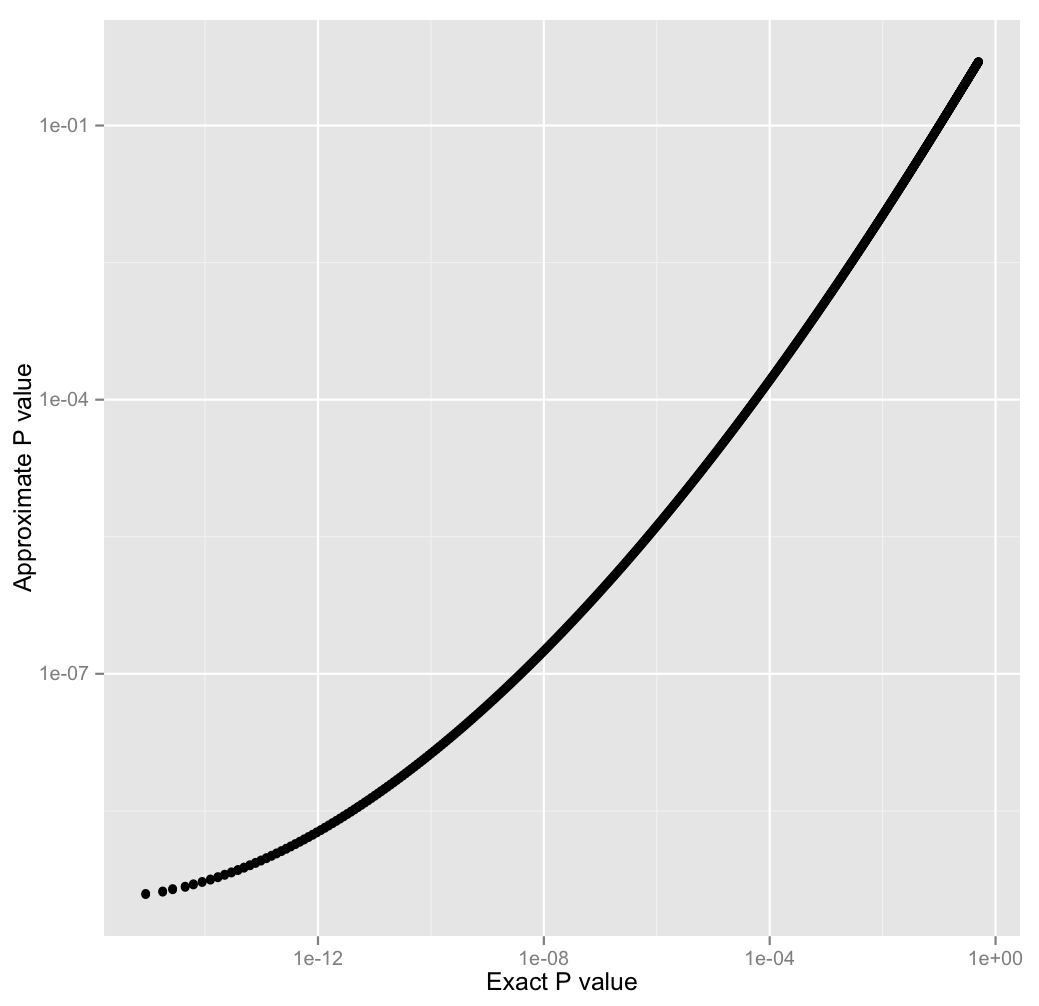
\includegraphics[width=0.8\textwidth]{PvsP50}
  \caption{P range with DRC algorithm when N=500}
  \label{fig:PdivPapproxDrcWhenN500}
\end{figure}

\subsection{Linear approximation}

\subsubsection{Goal}

Since we did not want to do anything really clever, we used linear approximation as the second alternative. Our goal is to drop as many intermediate points as we can, if they can be approximated with reasonable relative precision using linear interpolation.

\subsubsection{Linear approximation}
The linear approximation algorithm works by starting from data point in the data range and then one by one moving to the next data point, until the points between them cannot be approximated with enough accuracy. Then the last accurate point is saved, picked as the next starting point and the process is repeated until end of range has been reached. This guarantees approximated data range within error margin. The graphical illustration how linear approximation removes data points while approximating the general shape of the data array can be seen on the ~\ref{fig:linear_approximation}

\begin{figure}[H]
  \centering
  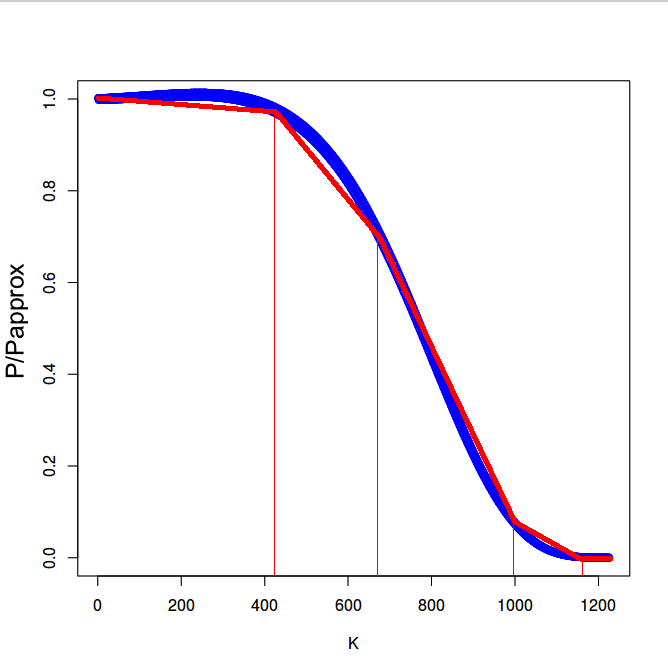
\includegraphics[width=0.8\textwidth]{linear_approximation}
  \caption{Linear approximation removing data points while staying within a certain error threshold and taking the general data array shape}
  \label{fig:linear_approximation}
\end{figure}

\subsubsection{Linear interpolation}
To reverse the algorithm, a very simple formula - linear interpolation is used.\\
Let $x$ be the approximated point $k$\\
Let $x_1$ be the start points $k$\\
Let $x_2$ be the end points $k$\\
Let $y_1$ be the start points p-value \\
Let $y_2$ be the end points p-value\\
Let $y$ be the approximated p-value.

\begin{equation}
  y = y_1 + \frac{(y_2 - y_1) * (x - x_1)}{(x_2 - x_1)}
\end{equation}

A graphical explanation of the algorithm can be seen on the Figure ~\ref{fig:linear_interpolation}

\begin{figure}[H]
  \centering
  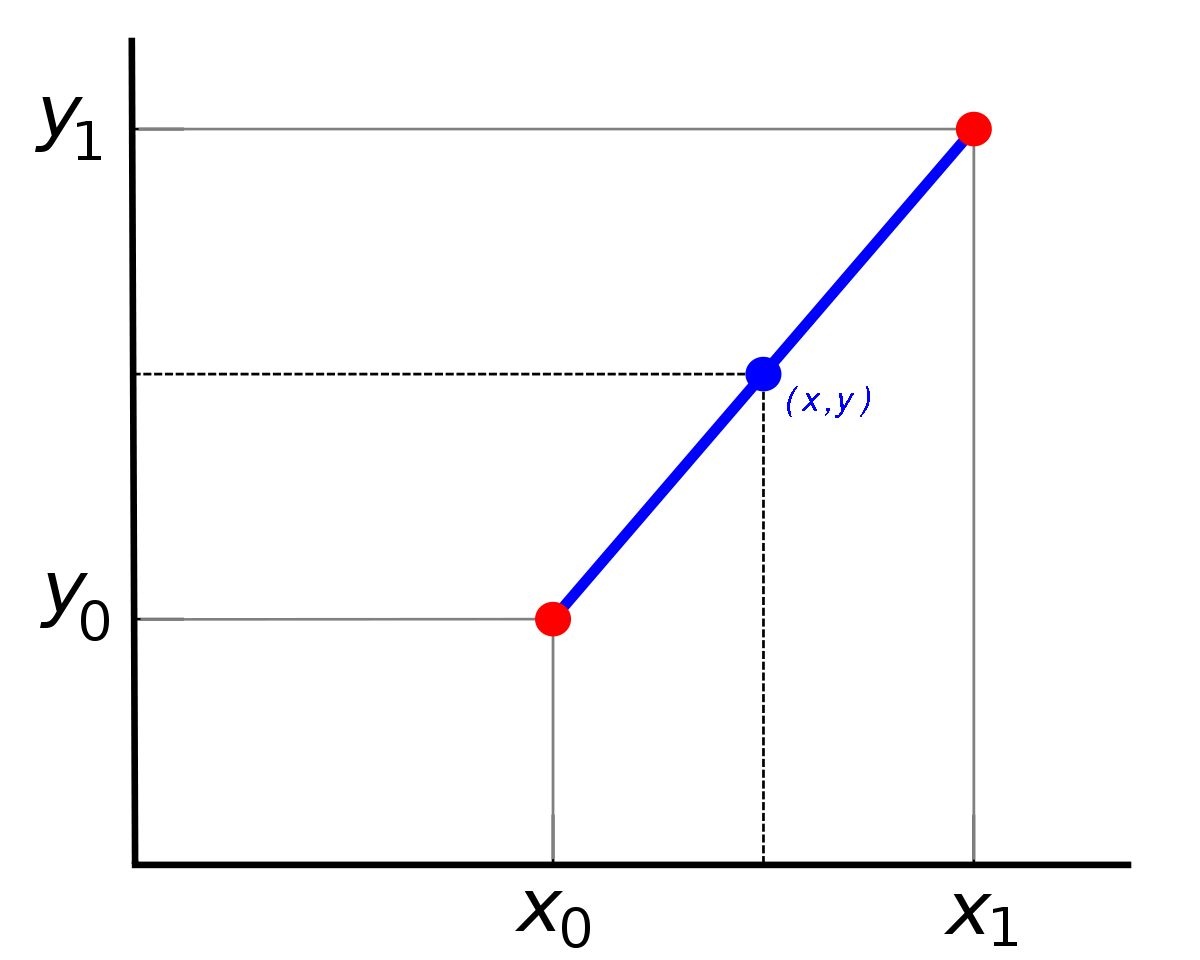
\includegraphics[width=0.8\textwidth]{linear_interpolation}
  \caption{Linear interpolation finding $y$, when given $x$, start point and end point ~\cite{linear_interpolation}}
  \label{fig:linear_interpolation}
\end{figure}

\subsubsection{Algorithm for dropping intermediate points}

The Linear approximation algorithm for dropping the data points in python looks like follows.

\begin{verbatim}
def linearInterpolate(approximatePoint,
                      endPoint,
                      startPoint,
                      endValue,
                      startValue):
  return startValue +
          ((endValue - startValue) * (approximatePoint - startPoint) /
          (endPoint - startPoint))

def canApproximate(actualPoints, currentPoint, nextPoint):
  startValue = actualPoints[currentPoint]
  endValue = actualPoints[nextPoint]

  for i in range(1, nextPoint - currentPoint):
    approximatePoint = currentPoint + i
    trueValue = actualPoints[approximatePoint]
    approximateValue = linearInterpolate(approximatePoint,
                                          currentPoint,
                                          nextPoint,
                                          startValue,
                                          endValue)
    if approximateValue == 0:
      return True

    relativeaccuracy = trueValue / approximateValue

    if relativeaccuracy < 0.9 or relativeaccuracy > 1.1:
      return False
  return True

def getNextApproximatedPoint(actualPoints, currentPoint):
  nextPoint = currentPoint + 1

  while(canApproximate(actualPoints, currentPoint, nextPoint)):
    if(nextPoint == len(actualPoints) - 1):
      break
    nextPoint += 1
  return nextPoint

def calculateApproximateRow(actualPoints):
  approximatedPoints = []
  currentPoint = 0
  approximatedPoints.append([currentPoint, actualPoints[currentPoint]])

  while(currentPoint != len(actualPoints) - 1):
    nextPoint = getNextApproximatedPoint(actualPoints, currentPoint)
    approximatedPoints.append([nextPoint, actualPoints[nextPoint]])
    currentPoint = nextPoint
  return approximatedPoints

\end{verbatim}

\subsection{Optimization summary}
The tests showed that using relative $P$ values between the $P$ tables gave less approximated data points, then using straight forward accurate $P$ table. In the end, thanks to linear approximation, the approximated table, when $N=500$ was created. The error margin for the chosen approximated table was chosen to be $20\%$, since that was deemed as accurate enough. Its still a lot more accurate then Gaussian P table at the edges of the table. The approximated table is only 1.6 MB large. Smaller then when $N=80$ the accurate P table was, which was around 2.5 MB.

\subsection{Further optimizations}
A lot of further optimizations could be done on this subject, for example

\begin{enumerate}
\item The algorithm to approximate accurate P table could be improved.
\item The plain text file could be compressed.
\item The shared library algorithm implementations could be improved and expanded.
\end{enumerate}

\newpage

\section{The implementation}

\subsection{Library description}
The implemented library consist of a C++ shared library, C++ terminal interface and R extended with C++ interface package.

The entire repository takes 8.1 MB, the shared library size is 1.9 MB, the terminal interface takes 1.9 MB, R interface takes 713 KB of disk space.

The performance tests show that the shared library could run over 20000 Wilcoxon tests with 120 samples in under 0.7 seconds. Compared to the vanilla R implementation which took many seconds to run 20 tests, this is a significant improvement.

\subsection{Repository description}

Repository that contains everything about our findings can be found in git repository ~\cite{wilx_repo}. The repository contains a number of folders.

\paragraph{WilcoxonTestLibrary}
Implementation for the optimized Wilcoxon test. The library can be installed by going to the WilcoxonTestLibrary folder and running the command
\begin{lstlisting}
$make install
\end{lstlisting}

\paragraph{RcppWilcoxonTest}
An interface that connects our implementation of the optimized Wilcoxon algorithm to the R. Note that you must have installed WilcoxonTestLibrary to use it. The interface must be compiled with separate R commands from the command line. You need Rcpp packages for R to use it. It can be installed in R console by running:
\begin{lstlisting}
$install.packages("Rcpp")
\end{lstlisting}

After that, the our Wilcoxon signed-rank implementation package can be installed to R by going to the RcppWilcoxonTest folder and running the command in the command line in the folder:

\begin{lstlisting}
$R CMD INSTALL .
\end{lstlisting}

You can now open the R console and load our library by running the command:

\begin{lstlisting}
>library('RcppWilcoxonTest')
\end{lstlisting}

To invoke the Wilcoxon test function, run:

\begin{lstlisting}
>RcppWilcoxonTest::WilxTest(dataMatrix, testIndexes, controlIndexes)
\end{lstlisting}

\paragraph{TerminalWilcoxonTest}

An interface that connects our implementation of the optimized Wilcoxon algorithm to the R. To use the terminal Wilcoxon test, you must first install Wilcoxon Test Library. It currently only supports NetCDF file as input data. The folder also contain example NetCDF file and the help gives instructions how to use it. The interface can be compiled by going to the TerminalWilcoxonTest folder and running the command:
\begin{lstlisting}
$make
\end{lstlisting}

Further information on how to use it can be found out with the command
\begin{lstlisting}
$./WilcoxonTest --help
\end{lstlisting}

\paragraph{WilcoxonVTable}
Python program that can calculate $V$, $P$ and approximated $P$ tables, print them, create files of the tables and create a number of graphs on the tables. The python version used is 3. The main file is called main.py, which is in the WilcoxonVTable directory.

\subsection{NetCDF file format}
As we needed to make an interface for the terminal, so BIIT could read NetCDF data files, without going through R, we needed to understand the BIIT data structure. However, eventually we wound up making the data matrix column and row names are configurable.
At the writing of this paper, the BIIT group holds the data in the NetCDF file in the following format:

\textbf{BIIT data matrix}
\begin{itemize}
  \item double data(m, n) - the data matrix of m genes (variables) and n samples (experiments, patients, ...)
  \item string gene[m] - gene IDs
  \item string array[n] - sample IDs
\end{itemize}

\textbf{BIIT non-track metadata}
\begin{itemize}
  \item string \_\_FileFormat - EVDF format identifier string. Current value: ``ExpressView 1.1".
  \item string \_\_DatasetType - A string identifying the dataset type. This is used to extract data-specific parameters from a global configuration file. See datatypes.conf (ExpressViewConfigFiles) for allowed values.
  \item string[n] Organism - Organism (per column)
  \item string[n] MetadataOrder - Sometimes metadata (including column tracks) may be in a different order than columns in data. This variable is a permutation of the array variable, specifying the order of column variables. This field is deprecated and all column metadata is expected to be in array order in new datasets.
  \item string InvestigationTitle - short title for the dataset
  \item string ExperimentDescription - long description for the dataset
  \item string DatasetID - Optional Source-specific dataset identifier
  \item string DatasetLink - Optional A URL associated with the dataset
  \item string \_\_VariableLabel - Optional Custom variable type name for the dataset. Overriden by variable\_label in project configuration. (ExpressView)
Names of any other (optional, non-track) metadata variables must be prepended by two underscores. Additional variables may be mandated by a data type specification, see ExpressViewConfigFiles. Known specific variables:
  \item string \_\_Organism - ArrayExpress chip organism (ArrayExpress; as opposed to the source of biological material stored in Organism)
\end{itemize}

\textbf{BIIT tracks}

Tracks are all other variables whose name begins with an uppercase character, that are arrays of either string or double, with the size of their first dimension either m or n. The former are referred to asrow tracks and the latter as column tracks. These variables encode some information about either the rows or columns of the data matrix; e.g. ExpressView displays column tracks above the heatmap.

Examples:

string Chemotherapy[n]
string Local\ Relapse[n]
double RelativeVariance[m]
\newpage

\section{Conclusion}
We found out that Gaussian distribution tail edge grows larger apart from the $P_{N, k}$ as $N$ increases while the overall distribution grows more similar. In addition, we confirmed that if thousands of parallel tests are ran, then using approximation is not reliable and instead an accurate table of p-values must be used. Calculating that table is very expensive and thus we advice to pre-calculate the table for the program. However, the research shows that if 10 000 measurements are run under 5\% relative error, then the hardcoded $N$ should be over 1000. Table of that size would take many gigabytes of space and is impractical to use.

To get around that, we approximated the accurate $P$ table. This allowed us to significantly reduce the size of the file and thus increase the hardcoded $N$ that was implemented inside the library.

For the time being, we chose $N=500$, with $20\%$ error margin on the approximation. This is still significantly more accurate then Gaussian approximated table at the edges of the distribution. It will allow to make 1000 parallel measurement with 5\% error margin.

The library itself could run over 20000 parallel tests with 100 samples in under a second. It is a shared C++ library with currently implemented interfaces in GNU-R and Terminal.

Overall the research included some surprising results and can be considered a success.

\newpage

\bibliographystyle{alpha}
\bibliography{bachelor-thesis}

\appendix
\pagebreak

\section*{\small Non-exclusive licence to reproduce thesis and make thesis public}

I, Stenver Jerkku (date of birth: 10th of October 1990),

\begin{tabbing}
\= Xiii\=\kill
\>1. \> herewith grant the University of Tartu a free permit (non-exclusive licence) to:\\\\

\>1.1\>
\begin{minipage}[t]{14.2cm}
reproduce, for the purpose of preservation and making available to the public, including for addition to the DSpace digital archives until expiry of the term of validity of the copyright, and
\end{minipage}
\\\\
\>1.2
\begin{minipage}[t]{14.2cm}
make available to the public via the web environment of the University of Tartu, including via the DSpace digital archives until expiry of the term of validity of the copyright,\\

Paralell Wilcoxon Signed-rank tests\\

supervised by Sven Laur

\end{minipage}\\\\
\>2. \>I am aware of the fact that the author retains these rights.\\\\
\>3. \>
\begin{minipage}[t]{14.2cm}
I certify that granting the non-exclusive licence does not infringe the intellectual property rights or rights arising from the Personal Data Protection Act.
\end{minipage}\\
\end{tabbing}

\noindent
Tartu, 14.05.2014

\end{document}
